\subsection{Disposición y elementos que hay en Inventarium}
Empezaremos hablando de los servicios y las interfaces y cómo se presenta su contenido en el caso de los primeros.

\subsubsection{Interfaces}
Tenemos una interfaz por cada elemento que se encuentra en la base de datos.

\subsubsection{Services}
Los servicios pueden ser los que hayan dado más tipos de problemas a lo largo del desarrollo. Son los encargados de generar las consultas HTTP de las que hemos hablado en la sección anterior en el desarrollo de la API.
\\Tenemos tantos servicios como tablas en la base de datos quitando el de \textit{user} que sirve para iniciar sesión dentro de la aplicación.

\begin{figure}[h]
    \centering
    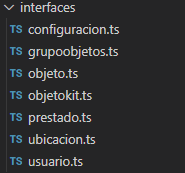
\includegraphics[keepaspectratio]{../contruccion_aplicacion/estructura_del_proyecto/interfaces.png}
    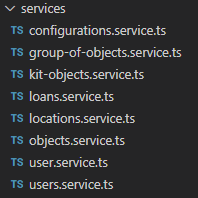
\includegraphics[keepaspectratio]{../contruccion_aplicacion/estructura_del_proyecto/servicios.png}
    \caption{Interfaces y servicios de UAL Inventarium}
\end{figure}

Para mostrar la estructura de uno de los servicios de la aplicación mostraré como ejemplo el fichero \textit{group-of-objects.service.ts}. Al principio del documento tendríamos las importaciones de código y más adelante declaramos lo siguiente:
\begin{verbatim}
    @Injectable({
        providedIn: 'root'
    })
\end{verbatim}
El \textit{@Injectable} junto al \textit{provideIn:`root'} sirve para que el servicio pueda utilizarse en todo el proyecto Angular.
\\Avanzando un poco más por el código nos encontramos con la declaración de nuestra variable \textit{\_url} a la cual le indicaremos la dirección a la que tiene que mandar la solicitud.
\begin{verbatim}
    _url = "api/grupoobjetos"
\end{verbatim}
Como vemos esa es la ruta a la que accederá a nuestra API. La dirección es así porque se ha habilitado un proxy que redirige las peticiones. De tal proxy se hablará más adelante.
\\En el constructor de nuestra aplicación inicializaremos la siguiente variable:
\begin{verbatim}
    constructor(private http: HttpClient) {}
\end{verbatim}
HttpClient es el servicio encargado de mandar las solicitudes HTTP a la API.
\\Ahora ya podemos empezar a crear las funciones que utilizaremos a lo largo del desarrollo:
\begin{verbatim}
    getGroupOfObjects() {
        return this.http.get(this._url);
    }
\end{verbatim}
En este caso la petición que se manda es del tipo \textit{get} si queremos crear un grupo de objetos sería así (con una petición \textit{post}):
\begin{verbatim}
    addGroupOfObject(objectGroup: FormData) {
        return this.http.post(this._url, objectGroup);
    }
\end{verbatim}
Donde como parámetro pasamos un campo del tipo formulario.
\\Para el resto de peticiones \textit{put} y \textit{delete} solamente le añadimos un campo numérico que sea la id del objeto que se va a modificar \textit{/:id} y en el caso de put también le pasamos otro tipo de objeto formulario.
\\Con esto ya tendríamos definido nuestro servicio y listo para funcionar.